\begin{figure*}[!t]
    \subfloat[平均端到端性能]{
        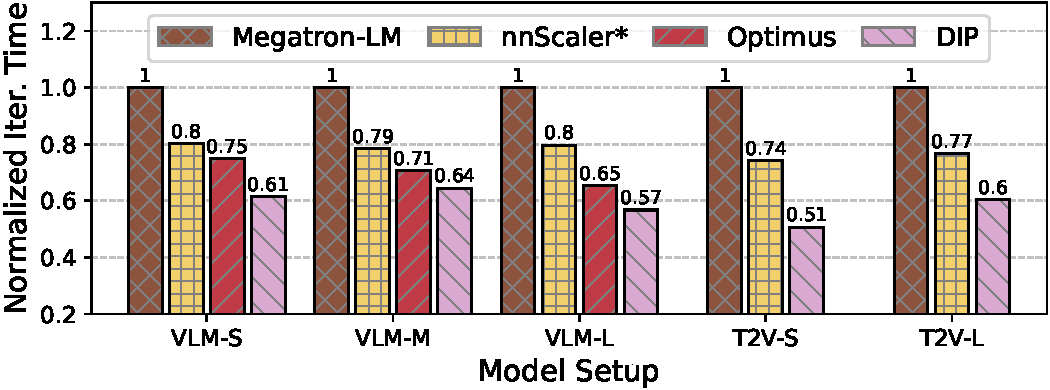
\includegraphics[height=29mm]{figures/weak_scaling.pdf}
    }
    \hfil
    \subfloat[动态工作负载]{
        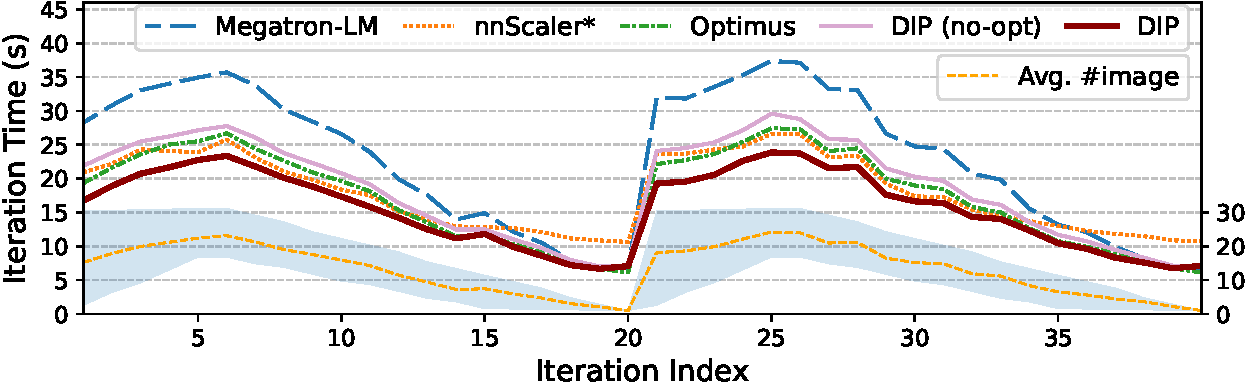
\includegraphics[height=29mm]{figures/dynamic_workload_timeline.pdf}
    }

    \caption{
        端到端性能。
        \textbf{(a)} 五种模型配置在真实数据集上运行 100 次迭代的平均性能。
        \textbf{(b)} 连续 40 次迭代的端到端延迟时间线。
        橙色虚线表示平均图像数量。
    }
    \label{figure:e2e-perf}
\end{figure*}

\section{评估}

\subsection{方法}
\label{section:datasets}

\heading{模型}
我们在两类主要 LMM 架构上全面评估 \sys{}：
视觉语言模型（VLM）和文本到视频（T2V）模型（\tableref{table:model-params}）。
VLM 架构将基于 ViT 的图像编码器（5B 和 22B 参数）~\cite{vit-iclr21,vit22b-arxiv23} 与语言模型骨干（Llama3 8B~\cite{llama3-arxiv24}、Qwen2 32B/72B~\cite{qwen2-arxiv24}）相结合；
T2V 架构则将语言模型编码器与基于 DiT 的扩散视频解码器（5B 和 30B 参数）~\cite{moviegen-arxiv24}相结合。
如\tableref{table:model-setup}所示，我们选择了五种不同的模型组合，其参数规模从 12B 到 94B。

\heading{数据集}
我们混合使用多个多样化的开源数据集~\cite{obelics-arxiv23,laion5b-nips22,scienceqa-nips22,share-gpt4-video-arxiv24,internvid-arxiv23,mmtrail-arxiv24}，
其中包括纯图文对、图文交错文档和视频--字幕对。
对于 VLM，我们采用 Qwen2 VL~\cite{qwen2-vl-arxiv24} 使用的 ViT 架构。我们将所有图像缩放至 728px 分辨率，每幅图像由 ViT 视觉编码器编码为 169 个 patch token（\texttt{patch\_size}=14，\texttt{spatial\_merge\_size}=4）。
多个图文数据样本被打包成 8192 token 的序列，因此每个序列最多容纳 $\lfloor 8192/169 \rfloor=48$ 幅图像。
对于 T2V 模型，我们采用 MovieGen~\cite{moviegen-arxiv24} 的配置，将视频转码为 16 FPS，最长时长为 16 秒。
处理短视频时，我们在每个微批次中最多组合 8 个视频片段，同时确保微批次总时长低于 16 秒。

\heading{基线}
我们将 \sys{} 与四个最先进基线系统进行比较：

\begin{itemize}
    \item \textbf{完全分片数据并行（FSDP）}~\cite{fsdp-arxiv23} 是 PyTorch 中标准的内存高效训练策略。它在数据并行工作进程之间分片模型参数、梯度和优化器状态，仅在计算当前层时通过通信收集这些数据。
    我们采用 PyTorch 2.8.0 中的 FSDP2，并为 Transformer 块使用 ZeRO-3 配置（\texttt{reshard\_after\_forward=true}），以尽量降低峰值内存使用量。
    \item \textbf{Megatron-LM}~\cite{megatron-lm-arxiv20} 是一种广泛使用的单模态 LLM 训练框架。
    我们采用交错流水线并行（VPP），并把 LMM 各层划分为参数分布大致均衡的模型块。
    \item \textbf{nnScaler}~\cite{nnscaler-osdi24}
    可自动完成深度神经网络训练的并行化。
    由于生成单个并行化计划需要数分钟，而且更新计划必须重启训练过程，
    我们在训练前使用有代表性的训练工作负载预先生成静态并行化计划。
    为公平比较不同框架，我们在 Megatron-LM 中实现了 nnScaler 的模型块划分方案和内存优化，
    并将性能指标标记为“nnScaler*”。
    \item \textbf{Optimus}~\cite{optimus-atc25}
    提出粗粒度和细粒度气泡调度，
    用于优化含多个编码器的多模态 LLM（MLLM）训练。
    粗粒度策略在流水线层面先依次执行所有模态编码器计算，再执行骨干模型；
    细粒度方法则用编码器计算填充 TP 通信气泡，
    与我们的流水线设计正交。
    为聚焦于流水线调度比较，我们在 \sys{} 中实现了 Optimus 的粗粒度气泡调度。
    由于 Optimus 不支持扩散解码器，我们在 T2V 模型评估中不纳入它。
\end{itemize}

评估未包含 Spindle~\cite{spindle-asplos25}，主要因为它针对静态多任务场景设计，要求在训练前预先定义任务。
这种静态设计与现代 LMM 所需的动态、灵活输入处理能力存在根本差异。

\heading{测试平台}
我们在一个由 8 个节点、共 64 块 NVIDIA 80GB H800 GPU 组成的集群上开展了大规模实验。
每个节点配有 128 个 CPU 核心、256GB 主机内存，
以及通过 200 GB/s NVLink 互连的 8 块 H800 GPU。
节点间通信使用采用 rail 优化拓扑的 8$\times$200Gbps RoCEv2 网络。
此外，我们还使用了一个较小的双节点集群与 FSDP 和 Megatron-LM 基线进行比较；每个节点配有 8 块 NVIDIA 96GB H20 GPU。

\heading{指标}\par\noindent
我们采用训练迭代时间和模型 FLOPs 利用率（MFU）作为性能指标，所有报告数值均取 10 次独立运行的平均值。

\subsection{端到端性能}
\label{section:e2e-performance}

\heading{与 LLM 训练系统比较}\par\noindent
我们首先将 {\sys} 与 FSDP 和 Megatron-LM 进行基准比较，
二者都是广泛使用的单模态 LLM 训练框架。
这些实验在 16-GPU H20 集群上开展，
利用每块 GPU 较大的 96GB 显存，尽量减少激活重计算开销。
如\tableref{table:fsdp-comparison}所示，
FSDP 仅比 Megatron-LM 慢 3\%，
而 {\sys} 相比 Megatron-LM 加速 27\%。
鉴于 FSDP 与 Megatron-LM 的性能差距很小，
我们基于 Megatron-LM 实现其余所有基线，以确保跨框架比较公平。

\begin{table}[t]
    \caption{
        FSDP、Megatron-LM 和 {\sys} 在 16 块 H20 GPU 上的 VLM-S 端到端性能。
    }
    \label{table:fsdp-comparison}

    \small
    \begin{tabular}{>{\raggedright}lccc}
    \toprule
    & \textbf{FSDP}~\cite{fsdp-arxiv23} & \textbf{Megatron-LM}~\cite{megatron-lm-arxiv20} & \textbf{\sys} \\
    \midrule
    迭代时间（s） & 40.270 & 39.053 & 28.606 \\
    相对时间 & 1.03 & 1.00 & 0.73 \\
    \bottomrule
    \end{tabular}
\end{table}

\heading{与多模态训练系统比较}
我们使用真实数据集和\tableref{table:model-setup}汇总的五种模型配置，将 \sys{} 的平均端到端性能与基线系统进行比较。
如\figref{figure:e2e-perf}a 所示，在 VLM 模型配置中，\sys{} 相比三个基线系统将训练吞吐量提高 15.6\%--76.2\%；
在 T2V 模型配置中，相比两个基线将训练吞吐量提高 36.6\%--97.3\%。
这说明其性能增益在不同模型架构和参数规模上保持一致。

\heading{动态工作负载}
为分析动态工作负载下 \sys{} 相对于其他基线的性能特征，
我们在 VLM-S 模型的训练迭代中手动控制图像数量上下界。
我们监测了 40 次迭代，其中图像数量呈现两次“先升后降”的变化模式。
每种模式包括：
(1) 在上界保持为 32 的同时，将下界从 0 逐步提高到 16（迭代 1--5），平均图像数峰值达到 22；
随后 (2) 逐步将上下界都降为零（迭代 6--20）。

\figref{figure:e2e-perf}b 表明，\sys{} 在所有系统中始终具有更优性能。
在图像数量较多的阶段（迭代 1--10），
Megatron-LM 在模态模块和数据微批次之间出现显著的计算不均衡，
第 6 次迭代时相较 \sys{} 慢 52.9\%。
尽管 nnScaler 和 Optimus 都在一定程度上缓解了动态不均衡的影响，
它们仍比 \sys{} 慢 10.4\%。
当图像数量和上下界之差均减小（迭代 11--20）时，
训练工作负载逐渐接近纯语言任务，
\sys{} 与基线系统之间的性能差距随之缩小。
值得注意的是，nnScaler 仅限使用 1F1B 调度，因而必须将所有模态模块划分到同一个流水线段中；
当图像编码器工作负载减小时，这会造成显著的流水线不均衡，
使迭代 15--20 的性能下降 50.5\%。

\subsection{性能消融}

\heading{性能分解}
在 VLM-S 模型配置上，
我们将四个关键组件
（模态感知划分器、流水线阶段交错、流水线段重排和逐层内存优化）
依次集成到 Megatron-LM 上。
如\tableref{table:performance-breakdown}所示，
仅模态感知划分器就比 Megatron-LM 基线提高 17.3\% 的性能，
凸显了它在 LMM 训练中的关键作用。
在流水线调度搜索器的各项优化中，
相较 Megatron-LM 的默认流水线机制，流水线阶段交错带来显著的 21.6\% 性能提升。
之后，流水线段重排和逐层内存优化通过智能重排流水线段和自适应选择内存优化策略，
又将性能提高 23.9\%。
在\figref{figure:e2e-perf}b 中，我们直观比较了动态工作负载下模态感知划分器和流水线调度搜索器带来的改进；
其中标记为“\sys{} (no-opt)”的曲线排除了流水线调度搜索器的优化，用作二者分界。

\begin{table}[t]
    \caption{
        \sys{} 各项优化的量化影响。
    }
    \label{table:performance-breakdown}

    \small
    \begin{tabular}{>{\raggedright}p{4.5cm}cc}
    \toprule
    \textbf{技术} & \textbf{迭代时间（s）} & \textbf{$\Delta$\%} \\
    \midrule
    原始 Megatron-LM & 26.13 & 0.0\% \\
    \midrule
    + 模态感知划分器（\S\ref{section:modality-aware-partitioning}） & 22.27 & 17.3\% \\
    + 流水线阶段交错（\S\ref{section:stage-interleaving}） & 18.81 & 38.9\% \\
    + 流水线段重排（\S\ref{section:segment-reordering}） & 17.61 & 48.3\% \\
    + 逐层内存优化（\S\ref{section:memory-optimization}） & 16.05 & 62.8\% \\
    \bottomrule
    \end{tabular}
\end{table}

\heading{子微批次大小的影响}
我们使用 VLM-S 模型，测试从 4 到 32 的图像子微批次大小，并分别求得最佳和最差\footnote{我们反转流水线调度搜索器的优化目标、改为最大化迭代时间，从而得到最差流水线调度。}流水线调度，
以研究特定于模态的子微批次大小对流水线调度和 GPU 执行效率的影响。

对\figref{figure:pipeline-scheduling}的分析揭示了两个关键发现。
第一，较小的子微批次大小（4--12）将最佳与最差调度之间的性能差距从 15.4\% 显著缩小到 5.1\%。
方差收窄表明系统对调度配置的敏感性下降，
从而降低了得到最优流水线调度的难度。
第二，过小的子微批次（<8）由于 GPU 计算能力利用不足而出现收益递减，
与中等大小的批次相比，其迭代时间增加 12.1\%。
通过实证验证，我们发现子微批次大小为 12 时，流水线调度灵活性与硬件利用效率达到最佳平衡。

\begin{figure}[!t]
    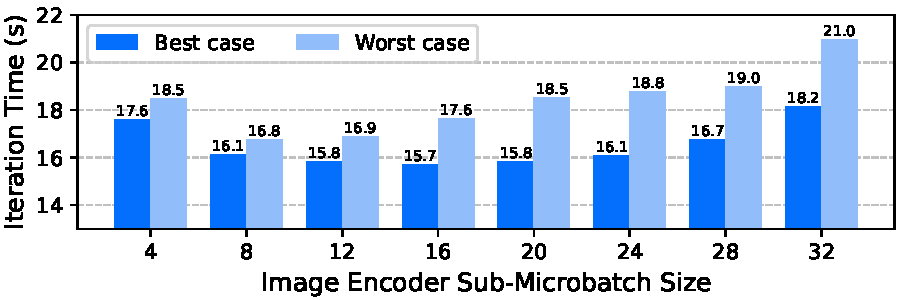
\includegraphics[width=1\columnwidth]{figures/pipeline_scheduling.pdf}
    \caption{
        子微批次大小的影响。
    }
    \label{figure:pipeline-scheduling}
\end{figure}

\heading{逐层内存优化的影响}
我们分析了 VLM-M 模型训练期间第一个流水线秩的内存使用时间线。
如\figref{figure:adaptive-computation}所示，
基线系统未能充分利用可用 GPU 内存。
Megatron-LM 在稳定的 1F1B 流水线阶段表现出显著的内存波动；
Optimus 则会先执行全部模态编码器计算并存储大量激活内存，因而内存使用逐步增加。
这使其峰值内存消耗比 Megatron-LM 高 25.3\%。
相比之下，\sys{} 将微批次拆分为更小的子微批次，
使前向和反向流水线阶段能够以更细粒度交错，
从而在整个训练迭代中始终保持较低的内存使用量。
逐层内存优化进一步智能选择内存优化配置，
以充分利用可用 GPU 内存；
相较 Megatron-LM，其内存波动减少 52.9\%，
并在峰值内存相同的条件下比 Optimus 获得 12.2\% 的性能增益。

\begin{figure}[!t]
    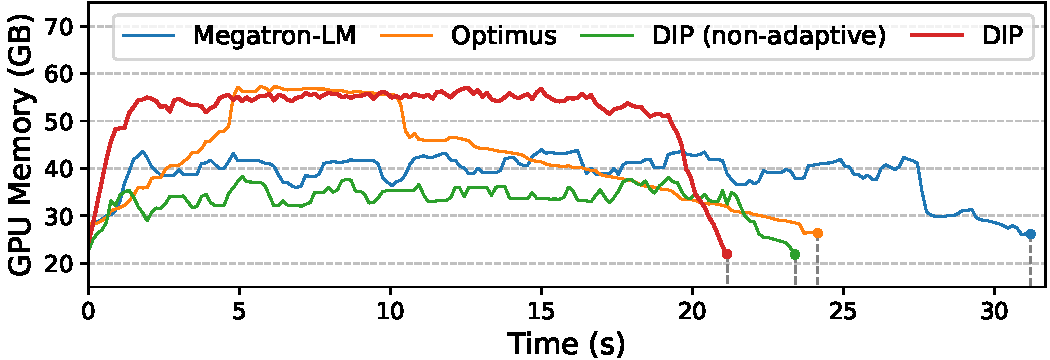
\includegraphics[width=1\columnwidth]{figures/adaptive_computation.pdf}
    \caption{
        VLM-M 训练中第一个流水线秩的内存使用时间线。
        “\sys{} (non-adaptive)”禁用了逐层内存优化，因而未使用全部可用 GPU 内存。
    }
    \label{figure:adaptive-computation}
\end{figure}

\begin{figure}[!t]
    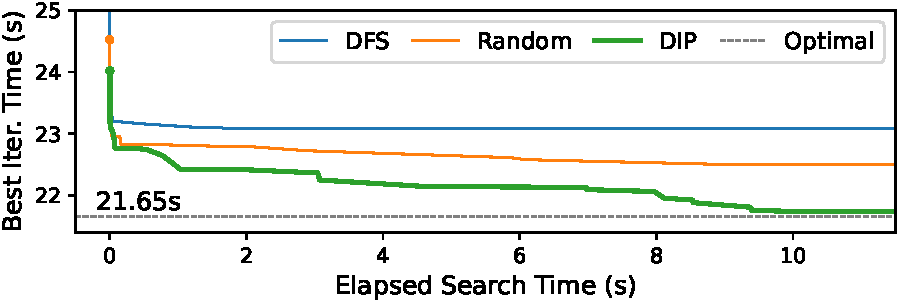
\includegraphics[width=1\columnwidth]{figures/search_efficiency.pdf}
    \caption{
        不同探索策略的搜索进展。
    }
    \label{figure:search-efficiency}
\end{figure}

\subsection{规划器评估}
\label{section:planner-evaluation}

\heading{搜索效率}
为展示 \sys{} 流水线调度搜索的效率，
我们跟踪当前最佳流水线调度性能随搜索时间的变化，
并与两个分别以深度优先搜索（DFS）和随机探索
替代 MCTS 算法的变体进行比较。
以最大的 VLM-L 模型作为目标工作负载，我们在 64 个 CPU 核心上运行所有搜索算法变体。
\figref{figure:search-efficiency}显示，\sys{} 在 10 秒内即可获得接近最优的流水线调度性能；
这一搜索过程可以与 VLM-L 通常长达 20 秒的训练迭代重叠。
相比之下，DFS 和随机探索策略缺少像 MCTS 那样以性能分数为引导的搜索优化，
无法快速找到最优流水线调度。

\heading{搜索可扩展性}
我们使用 VLM-S 和 T2V-S 两种模型配置评估搜索可扩展性。
具体而言，我们测量微批次数量增加时 {\sys} 的搜索延迟；
微批次增加会相应增加流水线阶段数量和流水线调度复杂度。
我们将 {\sys} 与两个最先进 SMT/ILP 求解器 Z3~\cite{z3} 和 Gurobi~\cite{gurobi}（13.0 版）进行基准比较。
在实验设置中，{\sys} 和 Gurobi 最多使用 64 个 CPU 线程；
Z3 本身不支持多线程求解，因此仅使用单线程。
如\figref{figure:search-scalability}所示，{\sys} 始终将搜索时间保持在 10 秒以内。
相比之下，Z3 和 Gurobi 的搜索时间均随微批次数量呈指数增长。
因此，当微批次数量超过 10 时，两个求解器都无法在 30 分钟内完成求解，
不适合用于 LMM 训练中的动态流水线调度生成。

\begin{figure}[!t]
    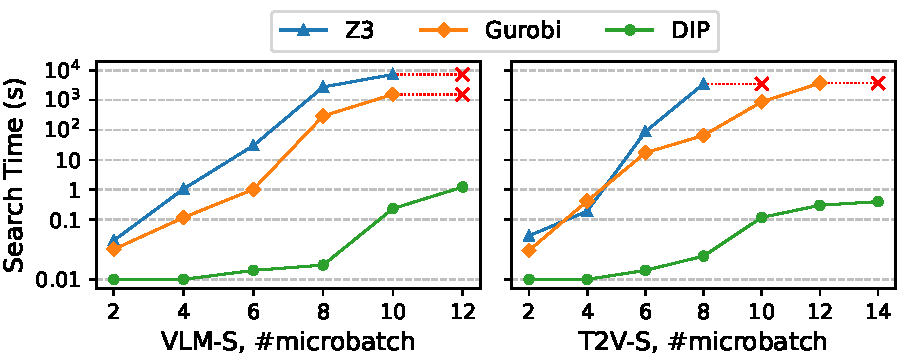
\includegraphics[width=1\columnwidth]{figures/search_scalability.pdf}
    \caption{
        在 VLM-S 和 T2V-S 上，Z3、Gurobi 与 {\sys} 面对不同微批次数量时的搜索时间比较。
        Y 轴采用对数尺度。
        红色叉号（\textcolor{red}{$\times$}）表示超时（>3 小时）。
    }
    \label{figure:search-scalability}
\end{figure}

\heading{仿真准确率}
我们通过 VLM-M 在 64 块 GPU 上的网格搜索实验评估 \sys{} 训练仿真器的准确率，
并将仿真结果与实际 GPU 执行结果进行比较。
我们系统评估了 DP、PP、TP 大小的所有有效组合，其中各数值均为 2 的幂，且 TP $\leq 8$。
如\figref{figure:simulation-accuracy}所示，最优并行配置为 DP8、TP2、PP4，MFU 达到 29.7\%。
尽管 \sys{} 的默认仿真设置与真实测量值相比，初始相对误差最高可达 10\%，
仿真器仍成功预测出了最优并行配置。
通过离线微基准校准矩阵乘法和集合通信操作的效率缩放因子，
训练仿真器达到平均 97.6\% 的仿真准确率。

\begin{figure}[!t]
    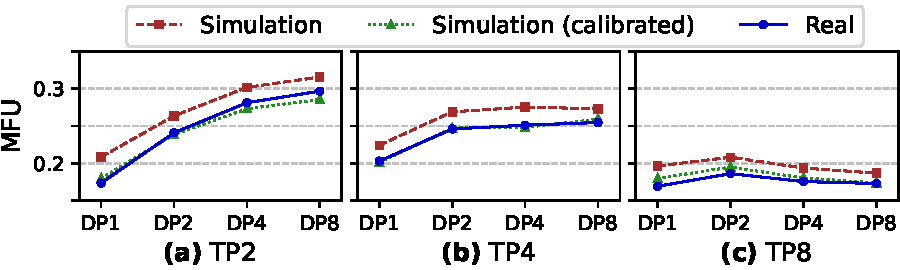
\includegraphics[width=1\columnwidth]{figures/simulation_accuracy.pdf}
    \caption{
        校准前后的仿真结果与实际 GPU 执行结果的比较。
    }
    \label{figure:simulation-accuracy}
\end{figure}

\subsection{大规模仿真}

为验证 \sys{} 在大规模 H100 GPU 集群环境中的有效性，
我们使用训练仿真器，针对两个规模庞大的大多模态模型（VLM-XL 和 T2V-XL）开展实验，
评估其相对于基线方法的理论改进。
两个模型和 GPU 集群的详细配置见\tableref{table:xl-model-setup}。

\begin{figure}[t]
    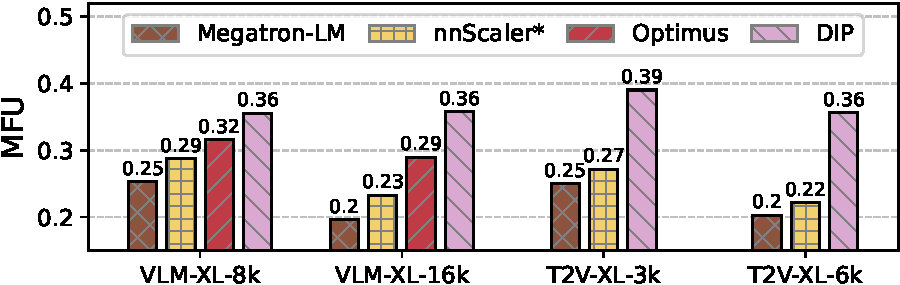
\includegraphics[width=1\columnwidth]{figures/large_scale_simulation.pdf}
    \caption{
        H100 集群上的大规模仿真。
    }
    \label{figure:large-scale-simulation}
\end{figure}

\heading{结果}
\figref{figure:large-scale-simulation}中的实验结果表明，\sys{} 在 VLM-XL 和 T2V-XL 上的 MFU 分别达到 0.36 和 0.39。
该系统始终优于基线方法，最高提升 82.8\%；
在流水线并行规模较大时优势尤为明显，
因为更大的 PP 维度会引入更复杂的流水线结构，
需要流水线调度搜索器对各阶段进行细致协调。
